\ifx\wholebook\relax \else

\documentclass{article}

\usepackage[nomarginpar
  %, margin=.5in
]{geometry}

\addtolength{\oddsidemargin}{-0.05in}
\addtolength{\evensidemargin}{-0.05in}
\addtolength{\textwidth}{0.1in}

\usepackage[en]{../prelude}

\setcounter{page}{1}

\begin{document}

\title{Paradox}

\author{Liu Xinyu
\thanks{{\bfseries Liu Xinyu} \newline
  Email: liuxinyu95@gmail.com \newline}
  }

\maketitle
\fi

\markboth{Paradox}{Mathematics of Programming}

\ifx\wholebook\relax
\chapter{Paradox}
\numberwithin{Exercise}{chapter}
\fi

\epigraph{I know that I know nothing}{——Socrates}

\begin{wrapfigure}{R}{0.5\textwidth}
 \centering
 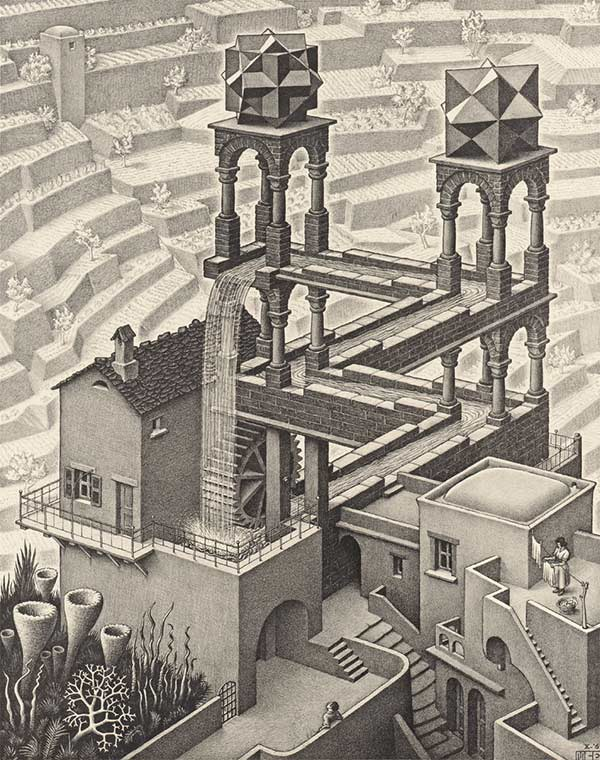
\includegraphics[scale=0.3]{img/Escher-Waterfall-1961.eps}
 \captionsetup{labelformat=empty}
 \caption{Escher, Waterfall, 1961}
 \label{fig:Escher-Waterfall}
\end{wrapfigure}

\index{Deep Blue}
In 1996, the 26th Summer Olympic game was hold in Atlanta, U.S. More than 10 thousand athletes from 197 nations challenges human limit of speed, strength, and team work in 26 sports. At the same time, there was another interesting match on-going. An IBM computer, called Deep Blue challenged the world chess champion Garry Kasparov in a six-game match. Deep Blue won the first game, but Kasparov won three and drew two, defeating Deep Blue by a score of 4:2. The next year, heavily upgraded Deep Blue challenged again to human world champion. On May 11, computer defected human: two wins for Deep Blue, one for the champion, and three draws. Deep Blue is a super computer of 1270 kilogram weight, with 32 processors. It can explorer 200 million possible moves in a second. The design team input 2 million grandmaster games in the past 100 years as the knowledge base for Deep Blue. The machine created by human intelligence, defected human at the first time in the field of intelligence. This result led to attention, fear, and hotly debating among mess media.

Most people believed this was a significant progress in artificial intelligence at that time. Although computer could defected human for chess, but there was still a big gap in board game Go. There are 8 rows and 8 columns in chess board, and 32 pieces. Computer need search among a big game tree containing about $10^{123}$ possible moves. Even Deep Blue could explore 2 million moves per second, it would take about $10^{107}$ year to exhaust the tree. The design team optimized the program to narrow down the search space, such that Deep Blue only need explore 12 moves ahead from current game. While the human grandmaster can only evaluate about 10 moves ahead. However for Go game, there are 19 rows and 19 columns, two players can put black and white pieces in 361 grids. The scale of the game tree is about $10^{360}$, which is far bigger than chess. For a long time after Deep Blue, people don't believe computer could defect human in Go.

%\begin{wrapfigure}{R}{0.5\textwidth}
\begin{figure}[htbp]
 \centering
 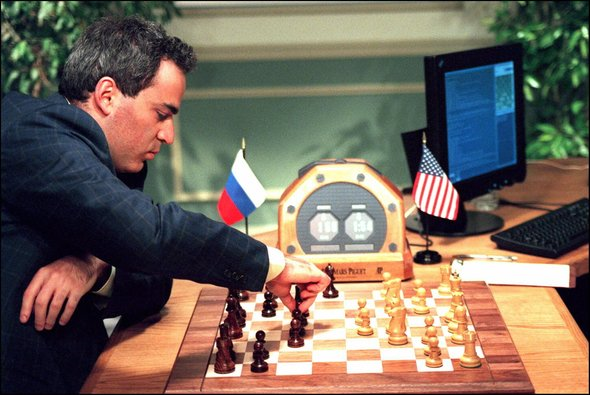
\includegraphics[scale=0.4]{img/Deep-blue-1997.eps}
 \captionsetup{labelformat=empty}
 \caption{Deep Blue versus Kasparov. from {\em Scientific American}}
 \label{fig:Deep-blue-1997}
\end{figure}
%\end{wrapfigure}

\index{AlphaGo}
20 years later in 2016, a computer program AlphaGo challenged top human go master. Korean professional 9-dan Go player, Lee Sedol, lost the game in a 1:4 series matches. One year after, the successor program AlphaGo master beat Chinese professional Ke Jie, the world number one ranked player, in a three-game match. Go had previously been regarded as a hard problem in artificial intelligence that was expected to be out of reach for the technology of the time. It was considered the end of an era. Facing the emotionless machine, Ke Jie was unwilling and burst into tears. As human beings, our feelings are mixed. Even the programmer community doing intellectual work is feeling the pressure from machine: will we be replaced by machine eventually?

%University of Tubingen, Germany
% Leon A. Gatys, Alexander S. Ecker Matthias Bethge
Traditionally, we thought the areas related to culture background, inner emotions, and human characters, like art, literature, and music could not be dominated by machine. In 2015, three researchers Gatys, Ecker, and Bethge from University of Tübingen, a small town 30 km south of Stuttgart, Germany applied machine learning to art style. By using deep convolutional neural network, they transformed a landscape photo of Tübingen into art painting of different styles\cite{Gatys-2015}. No matter the exaggerated emotion of the post-impressionist Van Gogh, or Turner's romantic turbid light and shadow effect, all vivid imitated by machine, as if the artists painted by themselves (figure \ref{fig:style-transfer}).

%\begin{wrapfigure}{R}{0.5\textwidth}
\begin{figure}[htbp]
 \centering
 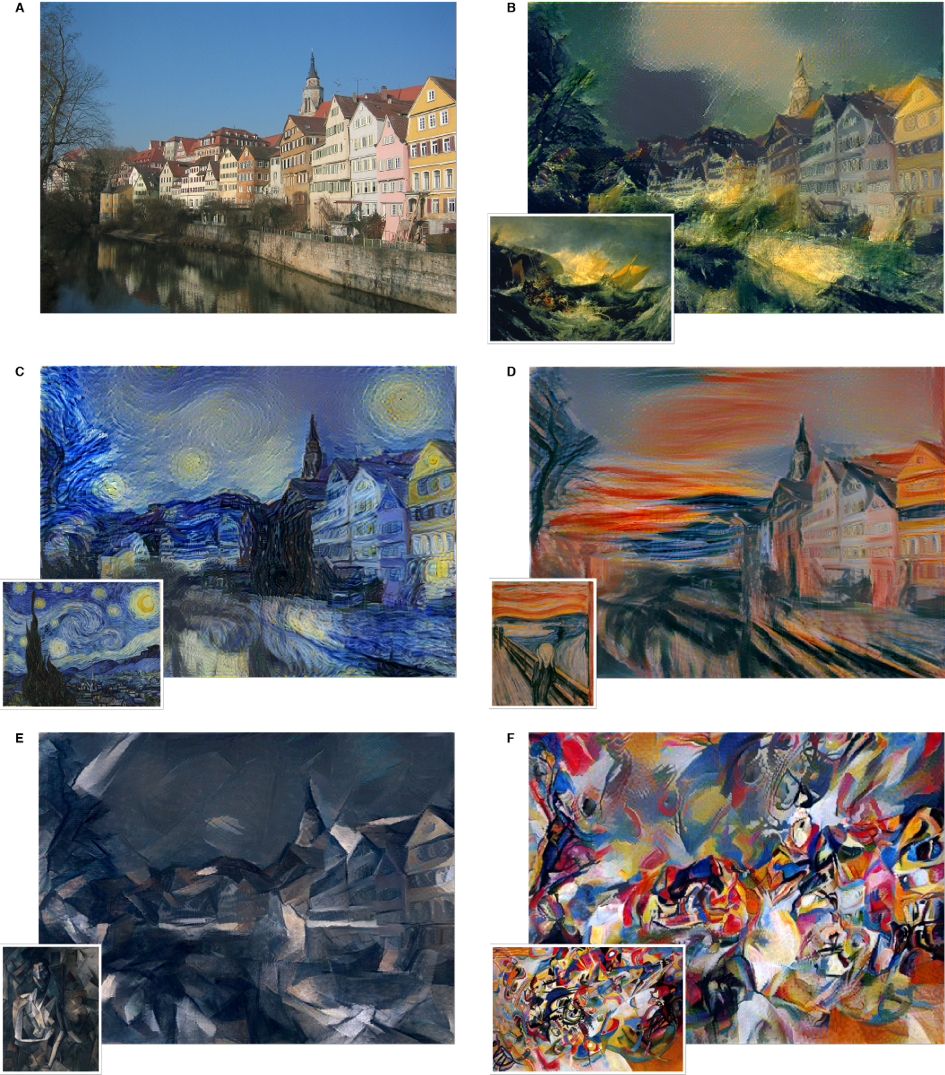
\includegraphics[scale=0.85]{img/style-transfer.eps}
 %\captionsetup{labelformat=empty}
 \caption{Artworks in different styles generated by machine learning: \textbf{A}, Landscape photo of Tübingen; \textbf{B}, {\em The Shipwreck of the Minotaur} by J.M.W. Turner, 1805; \textbf{C}, {\em The Starry Night} by Vincent van Gogh, 1889; \textbf{D}, {\em Der Schrei} by Edvard Munch, 1893; \textbf{E}, {\em Femme nue assise} by Pablo Picasso, 1910; \textbf{F}, {\em Composition VII} by Wassily Kandinsky, 1913.}
 \label{fig:style-transfer}
\end{figure}
%\end{wrapfigure}

In the following years, artificial intelligence and machine learning conquered varies of areas in a accelerated speed. Machines generated different styles of music, and played them out with moods and rhythms of tension, relaxing, and so on. It's no longer the a monotonous electronic piano sound. Machine batch translated news and academic papers, and comparable to human professional translators. Machine processed X-ray photos, CT, and MRI medical images to diagonal diseases, and the accuracy exceeded human doctors. Self-driven cars, powered by artificial intelligence traveled on streets, successfully overtaking other vehicles and avoid pedestrians. Automated groceries suddenly appeared on the street, people can pick the products and walk out without being checked out by a cashier... As humans we can't stop asking: Are we eliminating jobs faster than we creating? Will human be replaced by machine completely? Will machine rule people in the future?

All these reduce to one question: does there exist boundary of computation? if yes, where is it?

\section{Boundary of computation}

Gu Sen described the hesitated feelings when facing a long-running program in his popular book {\em Fun of thinking}: Will this program finish? Shall I go on waiting or kill it? Is there a compiler could tell if your program will run endlessly (\cite{GuSen-2012} pp.228)?

\begin{quotation}
\itshape
Why not possible? It seems more realistic than time machine. We may see such a scene in a scientific film: a programmer typed something in the dark screen, then hit enter. A highlighted, bold warning popped up immediately ``Warn: the program with the given input will run forever. Continue? (Y/N)'' If this became true one day, what fantastic cool things will you do? Do you believe that I can make big monkey with it? I'll firstly use it to prove the Goldbach's conjecture. I can write a program, enumerate all even numbers one by one, examine if it is the sum of two prime numbers. If yes, then check the next even number, otherwise output the negative example and quit. The next thing is compile my program. Can't the compiler determine my program terminates or not in advance? If the magic compiler warns me that my program will run endlessly, haven't I proved Goldbach's conjecture? Or if the compiler tells me the program will terminate, doesn't it mean Goldbach's conjecture is falsehood? Either case, I'll be the first one that solve the Goldbach's conjecture, and leave my name in mathematical history. What's the next? I will modify that program to explore the twin primes, then compile it to see if there are really infinite many twin primes. And next, are there infinite many Mersenne primes? This is also an open question in number theory for a long time. I can easily solve it in this way. The $3x + 1$ conjecture? It's a piece of cake to write a ``proof program'' in a few minutes, then win the 500 dollars prize offered by Paul Erdős. There are enough mathematical open questions, I'll never worry about nothing to do. Martin LaBar in 1984 asked if a $3 \times 3$ magic square can be constructed with nine distinct square numbers. The award has accumulated to 100 dollars, 100 euros, and a bottle of champagne. Search ``Unsolved problems in mathematics'', filter those about discrete things, and with award in, then write a few programs to solve them all...
\end{quotation}

\index{Turning's halting problem}
In 1936, the pioneer of computer science and artificial intelligence, Alan Turing proved a general algorithm to determine an arbitrary computer program will finish running, or continue to run forever, cannot exist. A key part of the proof was a mathematical definition of a computer and program, which became known as a Turing machine. This problem is called {\em halting problem} today.

To prove the Turing's halting problem, we can use reduction to absurdity method. Suppose there exists a algorithm $halts(p)$, that can determine an arbitrary program $p$ terminates or not. First, we construct a never halting program:

\[
forever() = forever()
\]

This is a infinitely recursive call. Then a define a special program $G$\footnote{We intended to use $G$ for special meaning. It's the first letter of Gödel, exactly the same name for nondeterministic proposition in Gödel's incompleteness theorem.} as below:

\[
G() = \begin{cases}
halts(G) = \text{halt}: & forever() \\
\text{otherwise}: & \text{halt} \\
\end{cases}
\]

In program $G$, we utilize $halts(G)$ to examine whether $G$ itself will halt or not. If it halts, then we call $forever()$ to let it run forever. It exactly means $G$ will not halt in this case, hence $halts(G)$ should be false. However, according to the second clause, it will halt. Therefore $halts(G)$ should be true. whether $halts(G)$ is true or false, we obtain conflict result. Hence our assumption can't hold. There does not exit a general algorithm to solve the halting problem for all possible program input.

There is another method to prove halting problem in two steps(\cite{SICP} pp.268). Most are same except that $G$ accepts another argument $p$, it applies $p$ to itself, then passes to $halts$:

\lstset{frame=single}
\begin{lstlisting}
G(p) = if halts(p(p)) then forever() else 'Halted'
\end{lstlisting}

As the next step, let's see what will happen when pass $G$ to itself $G(G)$. If $halts(G(G))$ returns true, then it calls $forever()$, hence $G(G)$ never finishes. While it exactly means $halts(G(G))$ should returns false, hence the program enters the \texttt{else}, and halts. But it again means $halts(G(G))$ should return true. Whether halts or not, it leads to absurdity.

The halting problem clearly provides a non-computable problem. Breaking the bubble of all the above magic ideas. It reminds us about the proof of Cantor's theorem in previous chapter. We used quite similar method proved that for all sets, including infinite sets, their cardinalities are strict less than their power sets. Actually, halting problem is closely related to many interesting logic paradoxes.

\section{Russel's paradox}

% Eubulides of Miletus
The history of paradox came back to ancient Greece. We've introduced Zeno's paradoxes about infinity and continuity. Logic paradox is often an interesting problem, with strict reasoning and deduced to conflict result. About the fourth Century BC, the ancient Greek philosopher Eubulides of Miletus raised a proposition: ``I am lying'' how to determine if this declaration is true or false?

If this declaration is false, then what it states (lying) should be true, it conflicts; however if this declaration is true, since it states I am laying, hence it should be false and lead to conflict again. Whether what Eubulides said is true or not, it all falls into contradiction. This confusing problem is called `liar paradox'.

\index{liar paradox}
There is a variance of liar paradox, appeared as two separated statements:

\textbf{Achilles}: The tortoise is a liar, he always lies. Do not trust him.

\textbf{Tortoise}: Dear Achilles, you are honest, you always speaks truth.

Is it true or false for what the tortoise said? If the tortoise tells the truth, then what Achilles states is true. However, Achilles claims the tortoise is laying, it leads to contradiction. On the contrary, if the tortoise tells lie, then what Achilles says is wrong, hence the tortoise should be true. We end up with a wired-loop: whether the tortoise speaks truth or not, all leads to absurdity.

This two-segment liar paradox sometimes appears as a joke. You received a piece of note: ``The other side is nonsense.'' while when you flip to the other side, it writes: ``The other side is true.'' Which side is true? In a similar way, it reduces to contradiction.

Such paradox also appears in children's story. A lion caught a rabbit. He is so happy, that he promise the rabbit: If you can guess what I am going to do, I'll let you go; otherwise I'll eat you. The clever rabbit then answers: I guess you are going to eat me.

If the lion eats the rabbit, then the rabbit guesses correct. Then the lion should keep his promise to let the rabbit go. However, if he let the rabbit go, it means the rabbit guesses wrong. Hence the lion should eat the rabbit. The lion falls into the dilemma, he should neither eat the rabbit, nor let the rabbit go. We can imagine the rabbit silently runs away when the lion keeps deep thinking.

According to the legend, after ancient Greek army defected Persian, the king decided to do something kind to the captives -- let them chose the way to be killed. According to what the captive said, if it is true, then cut head off, otherwise hang. A clever captive said: ``I think you are going to hang me.'' If the king hangs him, then what the captive said is true. Hence he should be cut head according to the rule. But if cut his head off, then it does not follow what the captive said. Hence he spoke falsehood, and should be hanged. Whether cut head or hang, the king's rule will not be conducted correctly. Facing such struggled situation, the king did not only let this clever man go, but also released all captives.

\begin{wrapfigure}{L}{0.5\textwidth}
 \centering
 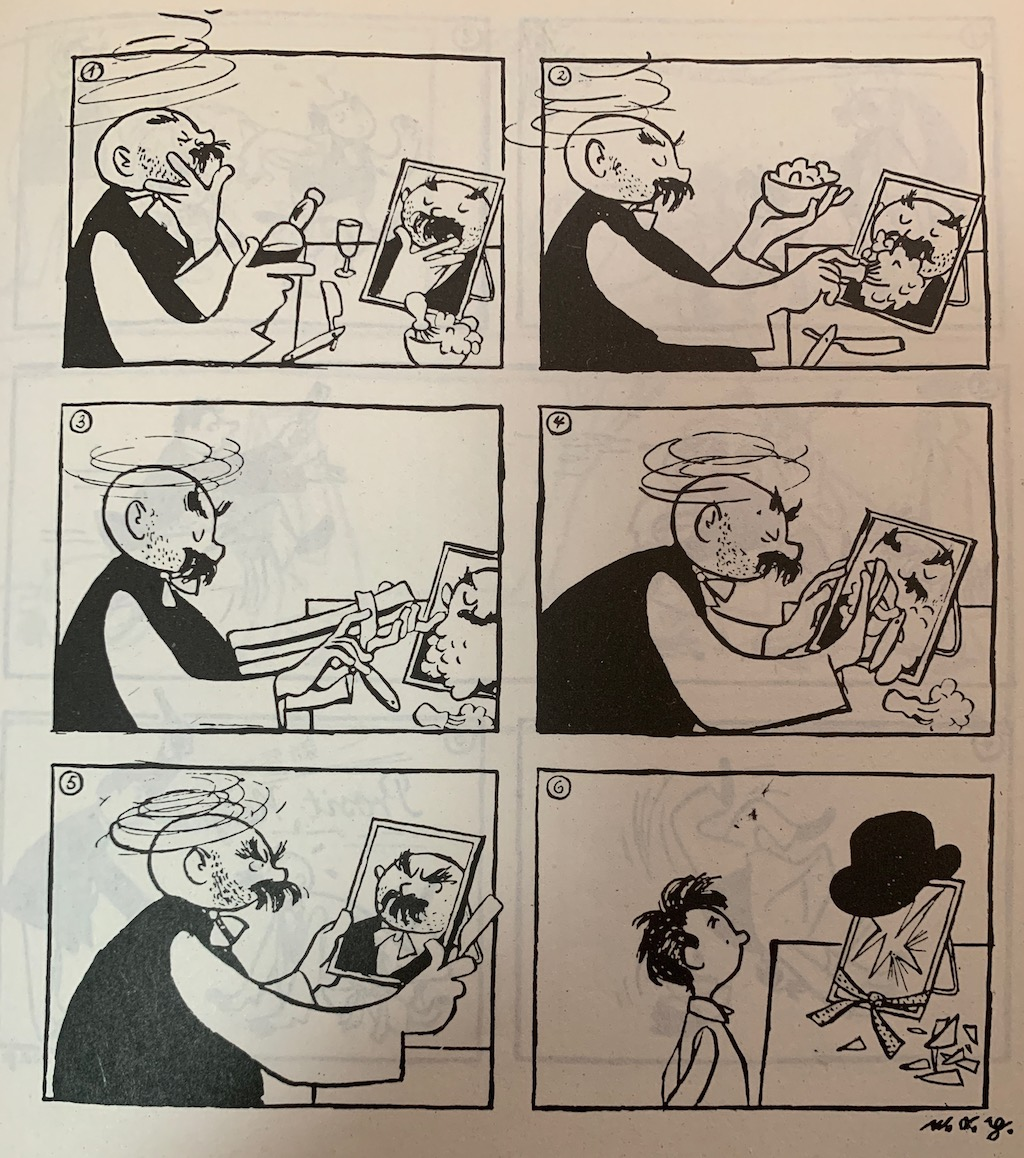
\includegraphics[scale=0.17]{img/father-and-son.eps}
 \captionsetup{labelformat=empty}
 \caption{E. O. Plauen {\em Father and Son}, 1930s}
 \label{fig:father-and-son}
\end{wrapfigure}

In Cervantes' novel {\em Don Quixote}, there is an interesting paradox in Part II, Chapter 51:

\begin{quotation}
\itshape
A deep river divides a certain lord’s estate into two parts... over this river is a bridge, and at one end a gallows and a sort of courthouse, in which four judges sit to administer the law imposed by the owner of the river, the bridge and the estate. It runs like this: ``Before anyone crosses this bridge, he must first state on oath where he is going and for what purpose. If he swears truly, he may be allowed to pass; but if he tells a lie, he shall suffer death by hanging on the gallows there displayed, without any hope of mercy.'' ... Now it happened that they once put a man on his oath, and he swore that he was going to die on the gallows there -- and that was all. After due deliberation the judges pronounced as follows: ``If we let this man pass freely he will have sworn a false oath and, according to the law, he must die; but he swore that he was going to die on the gallows, and if we hang him that will be the truth, so by the same law he should go free.''
\end{quotation}

% https://en.wikipedia.org/wiki/Barber_paradox
\index{Barber paradox}
Besides the liar paradox, the barber paradox is another popular puzzle. It was told by British mathematician and logician, Bertrand Russel in 1919. In a small village, the barber sets up a rule for himself: ``He only shaves all those, and those only, who do not shave themselves.'' Then the question is, does the barber shave himself? If he shaves himself, the according to his rule, she should not shave himself; but if he does not, then he should serve and shave himself. The barber falls into his own trap.

\index{Russell's paradox}
Russel discovered the paradox in set theory early in 1901. He collected and summarized a series of paradoxes, and formalize them as a fundamental problem in set theory. People called this kind of paradoxes as {\em Russell's paradox}. In Cantor's naive set theory, Russell considered the problem about if any set belongs to itself. Some sets do, while others do not. For example the set of all spoons is obviously not another spoon; while the set of anything that is not a spoon, is definitely not a spoon. Russell considered the latter, and extended it to all such cases. He constructed a set $R$, which contains all sets that are not members of themselves. Symbolically:

\[
R = \{ x | x \notin x \}
\]

Russell next asked, is $R$ a member of $R$? According to logical law of excluded middle, an element either belongs to a set, or does not. For a given set, it makes sense to ask whether the set belongs itself. But this well defined, reasonable question falls into contradiction.

If $R$ is a member of $R$, then according to its definition, $R$ only contains the sets that are not members of themselves, hence $R$ should not belong to $R$; On the contrary, if $R$ is not a member of $R$, again, from its definition, any set does not belong to itself should be contained, hence $R$ is a member of $R$. Whether it is a member or not, gives contradiction. Formalized as:

\[
R \in R \iff R \notin R
\]

Russell explicitly gave the paradox in Cantor's set theory.

\begin{wrapfigure}{R}{0.3\textwidth}
 \centering
 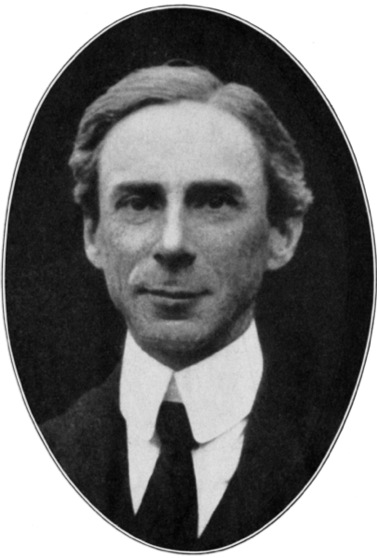
\includegraphics[scale=0.5]{img/Russell.eps}
 \captionsetup{labelformat=empty}
 \caption{Bertrand Russell, 1872 - 1970}
 \label{fig:Russell}
\end{wrapfigure}

%Monmouthshire
\index{Russell}
Russell was born in 1872 in Monmouthshire into a family of the British aristocracy. His mother died two years later, his father died when he was three. His grandfather died in 1878. His grandmother, the countess was the dominant family figure for the rest of Russell's childhood and youth. Her favourite Bible verse, ``Thou shalt not follow a multitude to do evil'', became his motto.

Russell was educated at home by a series of tutors. When Russell was eleven years old, his brother Frank introduced him to the work of Euclid, which he described in his autobiography as ``one of the great events of my life, as dazzling as first love.'' During these years, he read about the poems of Percy Bysshe Shelley, and think about religious and philosophy. In 1890, Russell won a scholarship to read for the Mathematical Tripos at Trinity College, Cambridge, where he became acquainted with Alfred North Whitehead. He quickly distinguished himself in mathematics and philosophy, graduating as seventh Wrangler in the former in 1893 and becoming a fellow in the latter in 1895.

Russell started an intensive study of the foundations of mathematics. He discovered Russell's paradox. In 1903 he published {\em The Principles of Mathematics}, a work on foundations of mathematics. It advanced a thesis of logicism, that mathematics and logic are one and the same. The three-volume {\em Principia Mathematica}, written with Whitehead, was published between 1910 and 1913. This, along with the earlier The Principles of Mathematics, soon made Russell world-famous in his field.

After the 1950s, Russell turned from mathematics and philosophy to international politics. He opposed nuclear war. The Russell–Einstein Manifesto was a document calling for nuclear disarmament and was signed by eleven of the most prominent nuclear physicists and intellectuals of the time. Russell was arrested and imprisoned twice. The second time he was in jail was at the age of 89, for ``breach of peace'' after taking part in an anti-nuclear demonstration in London. The magistrate offered to exempt him from jail if he pledged himself to ``good behaviour", to which Russell replied: ``No, I won't." In 1950 Russell won the Nobel Prize for Literature. The committee described him as ``in recognition of his varied and significant writings in which he champions humanitarian ideals and freedom of thought.''

Russell died of influenza on February 2nd, 1970 at his home in Penrhyndeudraeth. In accordance with his will, there was no religious ceremony; his ashes were scattered over the Welsh mountains later that year.

\subsection{Impact of Russell's paradox}

Russell was sad after discovering the paradox in the central of set theory. ``What makes it vital, what makes it fruitful, is the absolute unbridled Titanic passion that I have put into it. It is passion that has made my intellect clear, ... it is passion that enabled me to sit for years before a blank page, thinking the whole time about one probably trivial point which I could not get right ...''(\cite{HanXueTao16} pp.231) Russell wrote to mathematician, logician Gottlob Frege about his paradox. Frege was about to build the foundation of arithmetic. The second volume of his {\em Basic Laws of Arithmetic} was about to go to press. Frege was surprised, he wrote: ``Hardly anything more unwelcome can befall a scientific writer than that one of the foundations of his edifice be shaken after the work is finished. This is the position into which I was put by a letter from Mr Betrand Russell as the printing of this volume was nearing completion... '' Russell's paradox in axiomatic set theory was disastrous. Further, since set theory was seen as the basis for an axiomatic development of all other branches of mathematics, Russell's paradox threatened the foundations of mathematics. This motivated a great deal of research around the turn of the 20th century to develop a consistent (contradiction free) mathematics.

\begin{Exercise}
\Question{We can our natural language to define numbers. For example ``the maximum two digits number'' defines 99. Define a set of all numbers that can not be described within 20 words. Consider such an element: ``The minimum number that cannot be described within 20 words''. Is it a member of this set?}
\Question{``The only constant is change'' said by Heraclitus. Is this a Russell's paradox?}
\Question{Is the quote saying by Socrates a Russell's paradox?}
\end{Exercise}

\section{Philosophy of mathematics}

To solve Russell's paradox that affect the foundation of mathematics and logic, many mathematicians continued discussing, debating, and proposed varies of solutions from 1900 to 1930. For thousands of years, mathematics had long been regarded as the truth with non-doubtful absoluteness and uniqueness in rational thinking. In this hot discussion, people finally realized that different mathematics can coexist under different philosophical views.

\subsection{Logicism}

\begin{wrapfigure}{L}{0.3\textwidth}
 \centering
 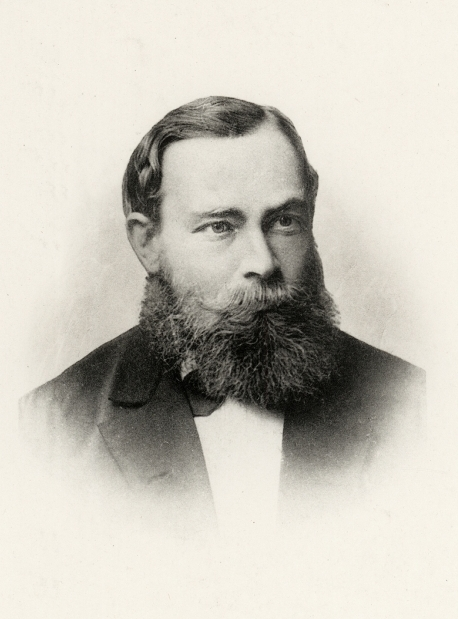
\includegraphics[scale=0.9]{img/Frege.eps}
 \captionsetup{labelformat=empty}
 \caption{Gottlob Frege, 1848-1925}
 \label{fig:Frege}
\end{wrapfigure}

\index{Frege}

Gottlob Frege was a German philosopher, logician, and mathematician. He is understood by many to be the father of analytic philosophy. Frege was the early representative of logicism. His goal was to show that mathematics grows out of logic, and in so doing, he devised techniques that took him far beyond the traditional logic. Frege treated the naive set theory as a part of logic. In order to do that, he defined natural numbers with logic. We know that numbers are abstraction from concrete things. For example 3 can represents three persons, three eggs, three angles in a figure and so on. All these collections are a {\em class}\footnote{Frege's work was prior to Cantor's, he used the term `class', while Cantor later used `set' in German} containing 3 elements. Which one should be used to represent natural number 3? Frege's idea is `all'. All the classes that 1-to-1 correspondence can be established to the above classes. This is a infinite, abstract class that defines natural number 3. Although a bit complex, it's a great definition that free from culture limitation. No matter what language, what symbol you are using, there won't be any ambiguities to understand number 3 through Frege's method. This is because no symbol is needed in Frege's definition. As such, Frege managed to define number -- which is the class of all classes. On top of this definition and logical laws, Frege developed his theory of natural numbers, hence established logical arithmetic. As the next step, he was going to develop all mathematics except for geometry from logic. This is what Frege wanted to achieved in his book {\em Basic Laws of Arithmetic}. Frege believed logical axioms were reliable and widely acceptable. Once his work completed, mathematics would be ``fixed on an eternal foundation''.

We know what happened next. Just during the preparation of press for {\em Basic Laws of Arithmetic}, Russell's letter arrived `in time'. Frege fell into confusions about Russell's paradox. His corner stone -- using logic to define the concept of numbers -- is exactly about class of all classes. Such definition directly leads to logical paradox. Frege was shocked, and finally gave up his logicism viewpoint.

Russell took over the torch of logicism. He then tried to reduce mathematics to logic in another way. Russell believed all mathematics is symbolic logic. His logicism was largely influenced by Italian mathematician Peano. In 1900, Russell attended the International Congress of Philosophy in Paris. He wrote: ``The Congress was the turning point of my intellectual life, because there I met Peano... In discussions at the Congress I observed that he was always more precise than anyone else, and that he invariably got the better of any argument on which he embarked. As the days went by, I decided that this must be owing to his mathematical logic... It became clear to me that his notation afforded an instrument of logical analysis such as I had been seeking for years...'' After came back, Russell and Whitehead discussed the basic concepts of mathematics every day. After hard work, they finally wrote the famous {\em Principia Mathematica}\footnote{Russell and Whitehead gave this Latin name in honor of Issac Newton's {\em Philosophiæ Naturalis Principia Mathematica}.}. The three volumes classic work about mathematical logic were published from 1910 to 1913. To solve the paradox, Russell pointed that: ``An analysis of the paradoxes to be avoided shows that they all result from a kind of {\em vicious circle}. The vicious circles in question arise from supposing that a collection of objects may contain members which can only be defined by means of the collection as a whole.'' He suggested: ``Whatever involves all of a collection must not be one of the collection'' and call this the ``vicious-circle principle''. To carry out this restriction, Russell and Whitehead introduced `theory of types'.

\begin{wrapfigure}{R}{0.4\textwidth}
 \centering
 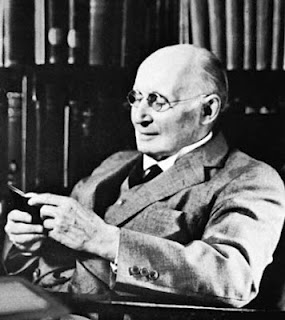
\includegraphics[scale=0.4]{img/Whitehead.eps}
 \captionsetup{labelformat=empty}
 \caption{Alfred North Whitehead, 1861-1947}
 \label{fig:Whitehead}
\end{wrapfigure}

\index{theory of types}
The theory of types classified sets into levels. Individual elements, such as a person, a number, or a particular book are of type 0; The sets of elements in type 0 are of type 1; The set of elements in type 1, which are sets of sets are of type 2... Every set is of a well defined type. The objects in a proposition must belongs to its type. Thus if one says $a$ belongs to $b$, then $b$ must be of higher type than $a$. Also one cannot speak of a set belonging to itself. Although this approach can avoid paradox, it is exceeding complex in practice. It took 363 pages till the definition of number 1 in {\em Principia Mathematica}, volume one. Poincaré remarked: ``eminently suitable to give an idea of the number 1 to people who have never heard it spoken of before.'' The theory of types requires all works at their proper type levels, propositions about integers have to be at the level of integers; propositions about rationals have to be at the level of rationals. $n/1$ and $n$ are at different levels, hence should not be handled in one proposition at the same time. And the common statements like ``all the real numbers...'' are not valid any more, as multiple types of sets are involved.

\index{约化公理}
The most questionable part is about {\em axiom of reducibility}, {\em axiom of choice}, and {\em axiom of infinity}. In order to handle natural numbers, real numbers, and transfinite numbers, Russel and Whitehead accepted the axiom of infinity to support the concept of infinite classes. They also accept one can chose elements from non-empty set or even infinite set to form new set. Such two arguable axioms exist in set theory too, however, many people opposed to the axiom of reducibility. To support mathematical induction, this axiom says any proposition at a higher level is coextensive with a proposition at type 0 level. Poincaré pointed out it was disguised form of mathematical induction. But mathematical induction is part of mathematics and is needed to establish mathematics. Hence we cannot prove consistency.

Later Russell himself became more concerned: ``Viewed from this strictly logical point of view, I do not see any reason to believe that the axiom of reducibility is logically necessary, which is what would be meant by saying that it is true in all possible worlds. The admission of this axiom into a system of logic is therefore a defect, even if the axiom is empirically true.''\cite{M-Kline-2007}

\subsection{Intuitionism}

\begin{wrapfigure}{L}{0.4\textwidth}
 \centering
 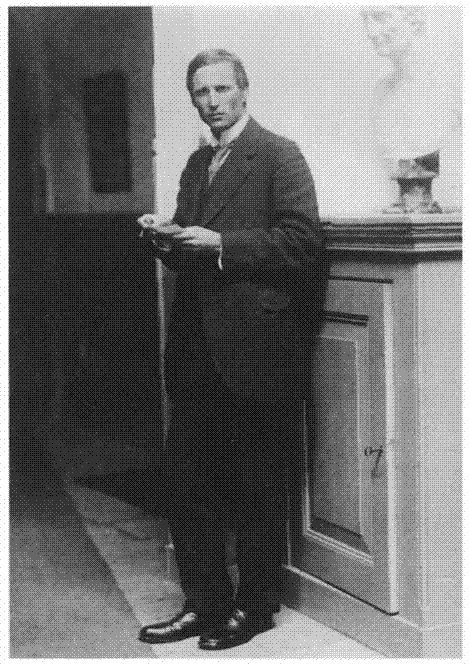
\includegraphics[scale=0.28]{img/Brouwer.eps}
 \captionsetup{labelformat=empty}
 \caption{L. E. J. Brouwer, 1881-1966}
 \label{fig:Brouwer}
\end{wrapfigure}

%图片来自The Low Countries, Arts and Society in Flanders and the netherlands. A year book 1998-99
\index{Brouwer}
On the contrary of logicism, some mathematicians took opposite approach to build the foundation of mathematics called intuitionism. They thought mathematics was purely the result of the constructive mental activity of humans rather than the discovery of fundamental principles claimed to exist in an objective reality. Intuitionism can be backtracked to Blaise Pascal. Kronecker we introduced in previous chapter was the pioneer mathematician hold intuitionism philosophy. Many world class mathematicians, including János Bolyai, Henri Lebesgue, Henri Poincaré, and Hermann Weyl support intuitionism. The founder is the Dutch mathematician Luitzen Egbertus Jan Brouwer. Brouwer was bore in 1881 in Overschie near Rotterdam, Netherlands. He entered University of Amsterdam in 1897, and soon demonstrated good mathematics capability. While still an undergraduate Brouwer proved original results on continuous motions in four dimensional space and published his result in the Royal Academy of Science in Amsterdam in 1904. Other topics which interested Brouwer were topology and the foundations of mathematics.

Influenced by Hilbert's list of problems proposed at the Paris International Congress of Mathematicians in 1900, Brouwer put a very large effort to study typology from 1907 to 1913. Among mathematicians generally, the best known is his fixed point theorem, usually referred to now as the Brouwer Fixed Point Theorem. This theorem states that in the plan every continuous function from a closed disk to itself has at least one fixed point. He also extended this theorem to arbitrary finite dimension. Specially, every continuous function from a closed ball of a Euclidean space into itself has a fixed point. In 1910, Brouwer proved topological invariance of degree, then gave the rigours definition of topological dimension. Because of the outstanding contribution to topology, he was elected a member of the Royal Netherlands Academy of Arts and Sciences.

When he was a post graduate student, he was interested in the on-going debate between Russell and Poincaré on the logical foundations of mathematics\footnote{Poincaré distinguished three kinds of intuition: an appeal to sense and to imagination, generalization by induction, and intuition of pure number—whence comes the axiom of induction in mathematics. The first two kinds cannot give us certainty, but, he says, ``who would seriously doubt the third, who would doubt arithmetic?''\cite{Poincare2}}. His doctoral thesis in 1907 attacked the logical foundations of mathematics and marks the beginning of the Intuitionist School. His views had more in common with those of Poincaré and if one asks which side of the debate between Russell and Poincaré he came down on then it would have with the latter. Brouwer was killed in 1966 at the age of 85, struck by a vehicle while crossing the street in front of his house.

Brouwer's intuitionism came from his philosophy: mathematics is a intellectual human activity. It does not exist outside our mind. Therefore, it is independent from the real physical world. The mind recognizes basic and clear intuitions. These intuitions are not perceptual or empirical, but directly admit certain mathematical concepts, like integers. Brouwer believed that mathematical thinking is a process of intellectual construction. It builds its own world, that is independent of experience, and is limited only by the basic mathematical intuition. The basic intuitive concepts should not be understood as undefined in axiomatic theory, but should be conceived as something, as long as they are indeed useful in mathematical thinking, they can be used to understand various undefined concepts in a mathematics.

\begin{wrapfigure}{R}{0.3\textwidth}
 \centering
 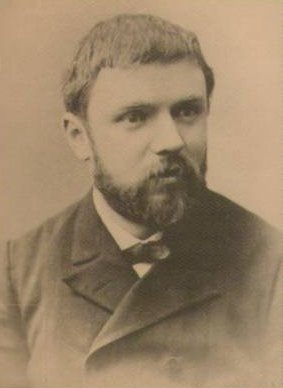
\includegraphics[scale=0.4]{img/Poincare.eps}
 \captionsetup{labelformat=empty}
 \caption{Henri Poincaré, 1854-1912}
 \label{fig:Poincare}
\end{wrapfigure}

In his 1908 paper, Brouwer rejected in mathematical proofs the principle of the excluded middle, which states that any mathematical statement is either true or false, no other possibility is allowed. Brouwer denied that this dichotomy applied to infinite sets. In 1918 he published a set theory, the following year a theory of measure, and by 1923 a theory of functions, all developed without using the principle of the excluded middle.

Brouwer's constructive theories were not easy to set up since the notion of a set could not be taken as a basic concept but had to be built up using more basic notions. Because of this, Intuitionism rejected non-constructive existence proofs. For example, Euclid's proof about the existence of infinite many prime numbers was not acceptable according to Brouwer because it does not give a way construct the prime number.

In general, intuitionism was more critical than construction in the first decades of the 20th Century. Intuitionism denied a large number of mathematical achievements, including irrational numbers, function theory, and Cantor's transfinite numbers. Many reasoning methods, like the principle of the excluded middle, were rejected. Therefore, it was strongly opposed by other mathematicians, Hilbert said: ``For, compared with the immense expense of modern mathematics, what would wretched remnants mean, the few isolated results incomplete and unrelated, that the intuitionists have obtained. ''

% Intuitionism enjoyed a resurgence of interest after World War II, primarily because of contributions by the American mathematician Stephen Cole Kleene.

\subsection{Formalism}

\begin{wrapfigure}{L}{0.5\textwidth}
 \centering
 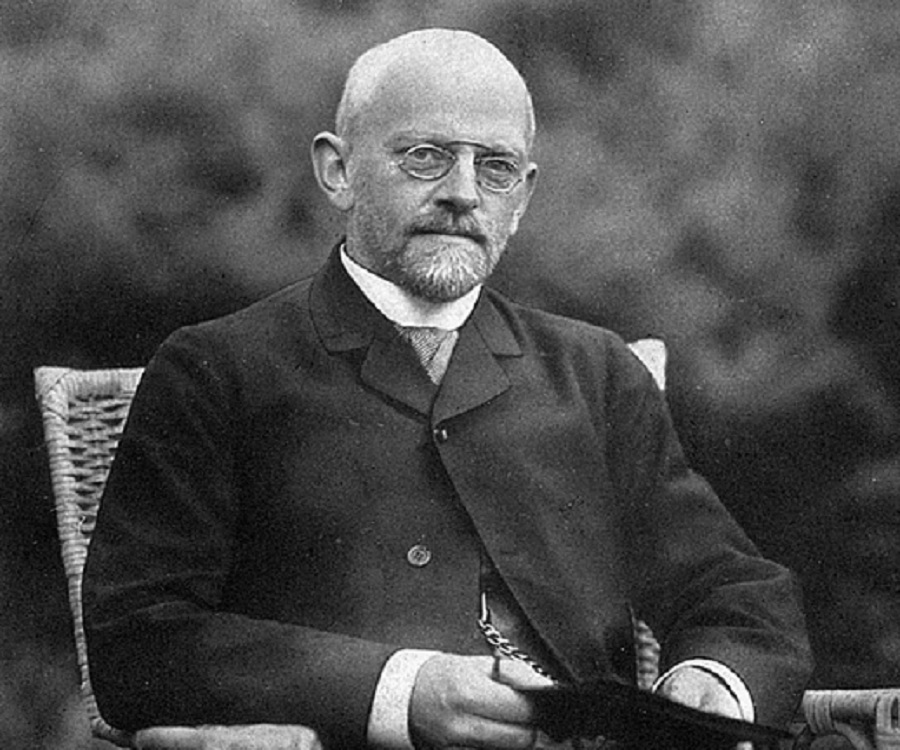
\includegraphics[scale=0.25]{img/Hilbert.eps}
 \captionsetup{labelformat=empty}
 \caption{David Hilbert, 1862-1943}
 \label{fig:Hilbert}
\end{wrapfigure}

\index{Hilbert}
The third mathematical school of thought is the Formalism led by the German mathematician David Hilbert. Hilbert was one of the most influential and universal mathematicians of the 19th and early 20th Centuries. He was born in 1862 in Königsberg, Eastern Prussia. He didn't shine at school at first, but later received the top grade for mathematics. In 1880, Hilbert enrolled at the University of Königsberg, where he met and developed lifelong friendship with Hermann Minkowski (two years younger than Hilbert), and associate professor Adolf Hurwitz (three years elder than Hilbert). Hilbert wrote: ``During innumerable walks, at times undertaken day after day, we roamed in these eight years through all the corners of mathematical science.''

In 1895, invited by Felix Klein, he obtained the position of Professor of Mathematics at the University of Göttingen. He remained there 48 years for the rest of his life. During the Klein and Hilbert years, Göttingen became the preeminent institution in the mathematical world. Students and young mathematicians viewed Göttingen as the Mecca of mathematics: ``Packed a bag and go to Göttingen!''

Hilbert contributed to many branches of mathematics. There are too many terms, theorems named after him, the even Hilbert himself did not know. He once asked other colleagues in Göttingen what `Hilbert space' was. ``If you think of mathematics as a world. which it is, then Hilbert was a world conqueror.''. When he died, {\em Nature} remarked that there was scarcely a mathematician in the world whose work did not derive from that of Hilbert.\cite{Ried-1996}

Hilbert put forth a most influential list of 23 unsolved problems at the International Congress of Mathematicians in Paris in 1900. This is generally reckoned as the most successful and deeply considered compilation of open problems ever to be produced by an individual mathematician. These were the problems which he considered most significant in mathematics at that time; not isolated questions but problems of such a general character that their solution was bound to have an enormous influence on the shape of future mathematics.
%cite: https://www.nature.com/articles/152182a0.pdf?origin=ppub
% Nature, Aug 14, 1943, Vol 52 pp. 182-183

Among Hilbert's students were Hermann Weyl, the famous world chess champion Emanuel Lasker, and Ernst Zermelo. But the list includes many other famour names including Wilhelm Ackermann, Felix Bernstein, Otto Blumenthal, Richard Courant, Haskell Curry, Max Dehn, Rudolf Fueter, Alfred Haar, Georg Hamel, Erich Hecke, Earle Hedrick, Ernst Hellinger, Edward Kasner, Oliver Kellogg, Hellmuth Kneser, Otto Neugebauer, Erhard Schmidt, Hugo Steinhaus, and Teiji Takagi. From 1933, the Nazis purged many of the prominent faculty members, included Hermann Weyl, Emmy Noether and Edmund Landau. About a year later, the new Nazi Minister of Education, Bernhard Rust asked whether ``the Mathematical Institute really suffered so much because of the departure of the Jews''. Hilbert replied, ``Suffered? It doesn't exist any longer, does it!'' Hilbert died in 1943 at age of 81. The epitaph on his tombstone in Göttingen consists of the famous lines he spoke: ``We must know. We will know.''

Hilbert's {\em Foundations of Geometry} published in 1899 proposes a formal set, called Hilbert's axioms, substituting for the traditional axioms of Euclid. It is the representative work of axiomatization. Hilbert's approach signaled the shift to the modern axiomatic method. From 1904, Hilbert started studying the foundation of mathematics. In 1920 he proposed explicitly a research project that became known as Hilbert's program. He wanted mathematics to be formulated on a solid and complete logical foundation. It opened the way for the development of the formalist school, one of three major schools of mathematics of the 20th century. According to the formalist, mathematics is manipulation of symbols according to agreed upon formal rules. It is therefore an autonomous activity of thought.

The main goal of Hilbert's program was to provide secure foundations for all mathematics. In particular this should include:

\begin{enumerate}
\item \textbf{A formulation of all mathematics}. In other words all mathematical statements should be written in a precise formal language, and manipulated according to well defined rules.

\item \textbf{Completeness}: a proof that all true mathematical statements can be proved in the formalism.
\item \textbf{Consistency}: a proof that no contradiction can be obtained in the formalism of mathematics. This consistency proof should preferably use only ``finitistic'' reasoning about finite mathematical objects.
\item \textbf{Conservation}: a proof that any result about ``real objects'' obtained using reasoning about ``ideal objects'' (such as uncountable sets) can be proved without using ideal objects.
\item \textbf{Decidability}: there should be an algorithm for deciding the truth or falsity of any mathematical statement.
\end{enumerate}

To execute his project, Hilbert initiated metamethematics, to study the mathematics itself using mathematical methods. This study produces metatheories, which are mathematical theories about other mathematical theories. Such approach actually differentiates three different mathematical systems:

\begin{enumerate}
\item None formalized Mathematics $G$: It's the normal mathematics, that allows classic logical reasoning. For example, applying principle of excluded middle on infinite set.

\item Formalized mathematics $H$: All symbols, formulas, axioms, and propositions are formalized. They are undefined concepts without any concrete meanings before explanation. Once explained, they are the concept in $G$. In other words, $G$ is the model of $H$, and $H$ is formalized $G$. As Hilbert described: ``One must be able to say at all times — instead of points, straight lines, and planes — tables, chairs, and beer mugs.'' With this approach, the specific meanings and background in Euclid geometry are put aside, we only focus on the relations between the undefined concepts, which are reflected through a collection of axioms.

\item Metamathematics $K$: This is the metatheories to study $H$. All reasoning in $K$ should be admitted intuitively. For example, without applying principle of excluded middle on infinite set.
\end{enumerate}

While Hilbert and the mathematicians who worked with him in his enterprise were committed to the project, a young mathematician Gödel proved incompleteness theorems, which showed that most of the goals of Hilbert's program were impossible to achieve. We'll explain the details in later sections.

\subsection{Axiomatic set theory}

Different from the mathematical schools of logicism, intuitionism, and formalism, the members of the set-theoretic school did not formulate their distinct philosophy at the beginning, but they gradually gained adherents, and a program. This school today earns as much as supporters as the other three we introduced.

The set-theoretic school can be traced back to Cantor and Dedekind's work. Although both were primarily concerned with infinite sets, they found by establishing the concept of natural numbers on basis of set, all of mathematics could then be derived. When Russell's paradox was found at the centre of Cantor's set theory, some mathematicians believed that the paradox was due to the informal introduction of sets. Cantor's set theory is often described today as `naive set theory'. Hence the set theoretic thought that a carefully selected axiomatic foundation would remove the paradoxes of set theory. Just as the axiomatization of geometry and of the number system had resolved logical problems in those areas. German mathematician Ernst Zermelo first took the axiomatization approach in set theory in 1908.

\index{Zermelo}
Zermelo also believed the paradoxes arose because Cantor had not restricted the concept of a set. He therefore stressed with clear and explicit axioms to clarify what is meant by a set, and what properties sets should have. In particular, he wanted to limit the size of possible sets. He had no philosophical basis but sought only to avoid the contradictions. His axiom system contained the undefined fundamental concepts of set and the relation of one set being included in another. These and the defined concepts were to satisfy the statements in the axioms. No properties of sets were to be used unless granted by the axioms. In his system, the existence of infinite sets, the operations as the union of sets, and the formation of subsets were provided as axioms. Zermelo also used the axiom of choice\cite{M-Kline-2007}.

\begin{figure}[htbp]
  \centering
  \subcaptionbox{Ernst Zermelo, 1871-1953}[0.45\linewidth]{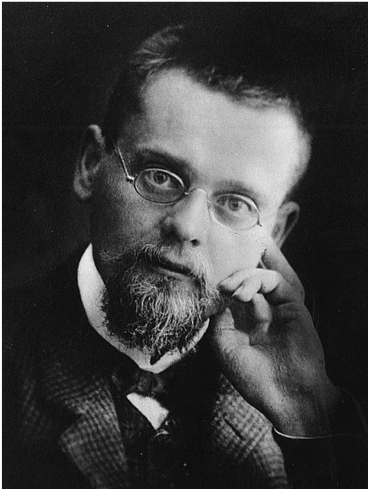
\includegraphics[scale=0.7]{img/Zermelo.eps}} \quad
  \subcaptionbox{Abraham Fraenkel, 1891-1965}[0.45\linewidth]{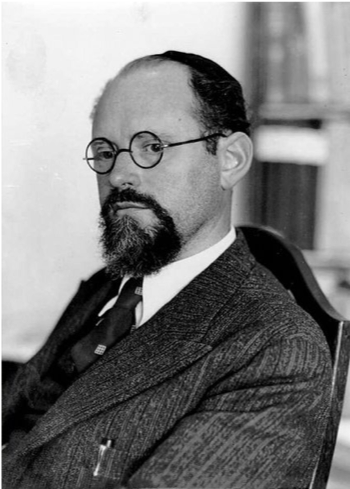
\includegraphics[scale=0.7]{img/Fraenkel.eps}}
  \captionsetup{labelformat=empty}
  \caption{}
  \label{fig:Zermelo-and-Fraenkel}
\end{figure}

\index{ZF system} \index{Fraenkel}
Zermelo's system of axioms was improved by Abraham Fraenkel in 1922. Zermelo did not distinguished a set property and the set itself, they were used as synonymous. The distinction was made by Fraenkel. The system of axioms used mostly common by set theorists is known as Zermelo-Fraenkel system, abbreviated as ZF system. They both saw the possibility of refined and sharper mathematical logic available in their time, but did not specify the logical principles, which they thought were outside of mathematics, and could be confidently applied as before\cite{M-Kline-2007}.

Zermelo provided 7 axioms in his 1908 paper. Then in 1930, Fraenkel, Skolem, and Von Neumann suggested to add another two axioms. These axioms are as below:

\index{axiom of choice}
\begin{enumerate}
\item \textbf{Axiom of extensionality}: Two sets are equal if they have the same elements. For set $A$ and $B$, if $A \subseteq B$ and $B \subseteq A$, then $A = B$.

\item \textbf{Empty set}: The empty set exists.

\item \textbf{Axiom schema of separation}: Also known as axiom schema of specification. Any property that can be formalized in the language of the theory can be used to define a set. For set $S$, if proposition $p(x)$ is defined, then there exists set $T = \{ x | x \in S, p(x)\}$.

\item \textbf{Axiom of power set}: One can form the power set (the collection of all subsets of a given set) of any set. This process can be repeated infinitely.

\item \textbf{Axiom of union}: The union over the elements of a set exists.

\item \textbf{Axiom of choice}:abbreviated as AC.

\item \textbf{Axiom of infinity}: There exists a set $Z$, containing empty set. For any $a \in Z$, then $\{a\} \in Z$. This axiom ensures infinite set exits.

\item \textbf{Axiom schema of replacement}: This axiom is introduced by Fraenkel in 1922. For any function $f(x)$ and set $T$, if $x \in T$, and $f(x)$ is defined, there exits a set $S$, that for all $x \in T$, there is a $y \in S$, such that $y = f(x)$. It says that the image of a set under any definable function will also fall inside a set.

\item \textbf{Axiom of regularity}: Also known as axiom of foundation. It was introduced by Von Neumann in 1925. $x$ does not belong to $x$.
\end{enumerate}

As such, set theory was abstracted to a axiomatic system. Set turned to be an undefined concept that satisfies these axioms. They do not permit `all inclusive set', hence avoid the paradox, and fixed the defects in naive set theory. However, there were still debate about which axioms were acceptable, particularly the axiom of choice is arguable.

%\begin{wrapfigure}{R}{0.5\textwidth}
\begin{figure}[htbp]
 \centering
 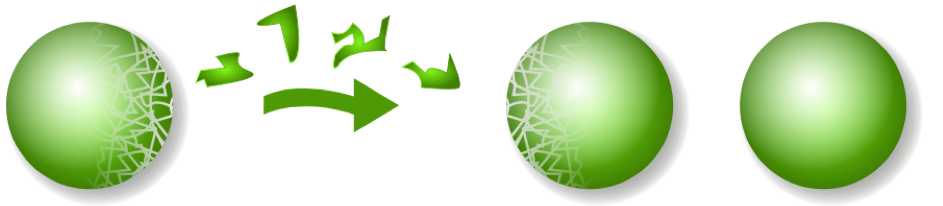
\includegraphics[scale=0.6]{img/Banach-Tarski-Paradox.eps}
 %\captionsetup{labelformat=empty}
 \caption{Banach-Tarski paradox: a solid ball can be decomposed and put back together into two copies of the original ball.}
 \label{fig:Banach-Tarski-Paradox}
\end{figure}
%\end{wrapfigure}

\index{Banach-Tarski paradox} \index{ZFC system}
In 1924, Polish mathematicians Stefan Banach and Alfred Tarski proved a theorem called Banach-Tarski paradox\footnote{Also known as Hausdorff-Banach-Tarski theorem, or `Doubling sphere paradox'.}. This theorem states that, if accept axiom of choice, then for a solid ball in 3 dimensional space, there exists a decomposition of the ball into a finite number of disjoint subsets, which can then be put back together in a different way to yield two identical copies of the original ball. Indeed, the reassembly process involves only moving the pieces around and rotating them without changing their shape. Banach and Tarski was going to reject axiom of choice through this theorem. However, their proof looked so natural, that mathematicians tend to consider it only reflects the counter intuitive fact about axiom of choice. Some set-theorists insist not to including axiom of choice, such axiomatic set theory is called ZF system, while the one included axiom of choice is called ZFC system. We introduced the interesting relation between axiom of choice and continuum hypothesis in previous chapter.

\section{Gödel's incompleteness theorems}

By 1930, there had been four separated, distinct, and more or less conflicting approaches about mathematics foundation. Their supporters adherence to their own mathematical schools. One could not say a theorem is correctly proven, because by 1930, he had to add by whose standard, it was proven correct. The consistency of mathematics, which motivated the these new approaches was not settled at all except if one argue that it's the human intuition guarantees consistency\cite{M-Kline-2007}. Hilbert was still planing his project optimistically to prove the completeness and consistency of mathematics. All these were ended up by a young mathematician and logician, Gödel.

\begin{wrapfigure}{L}{0.4\textwidth}
 \centering
 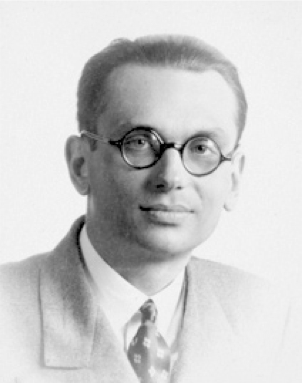
\includegraphics[scale=0.8]{img/Godel-young.eps}
 \captionsetup{labelformat=empty}
 \caption{Kurt Gödel, 1906-1978}
 \label{fig:Godel-young}
\end{wrapfigure}

\index{Gödel}
Kurt Gödel was born in 1906 in Brünn, Austria-Hungary Empire (now Brno, Czech Republic) into the German family. He had quite a happy childhood. He had rheumatic fever and recovered at age 6. However, 2 years later when read medical books about the illness, he learnt that a weak heart was a possible complication. Although there is no evidence that he did have a weak heart, Kurt became convinced that he did, and concern for his health became an everyday worry for him. In his family, young Kurt was known as ``Mr. Why'' because of his insatiable curiosity.

In 1924, Gödel entered the University of Vienna. he hadn't decided whether to study mathematics or theoretic physics until he learnt number theory. He decided to take mathematics as his main subject in 1926. Gödel was also interested in philosophy, and took part in seminars about mathematical logic. The exploration of philosophy and mathematics set Gödel's life course.

In 1929, at the age of 23, he completed his doctoral dissertation. In it, he established his completeness theorem regarding the first-order predicate calculus. He was going to further study Hilbert's program to prove the completeness and consistency of mathematics in finite steps. However, he soon developed an excepted result. In 1930 Gödel attended the Second Conference on the Epistemology of the Exact Sciences, held in Königsberg. Here he delivered his first incompleteness theorem, and soon, proved the second incompleteness theorem.

Gödel worked at University of Vienna from 1932. In 1933, Adolf Hitler came to power in Germany, the Nazis rose in influence in Austria academy over the following years. In 1936, Moritz Schlick, whose seminar had aroused Gödel's interest in logic, was assassinated by one of his former students. This triggered ``a severe nervous crisis'' in Gödel. He developed paranoid symptoms, including a fear of being poisoned. After the world war II broken out, Gödel accepted the invitation from the Institute for Advanced Study in Princeton, New Jersey. and moved to US. To avoid the difficulty of an Atlantic crossing, the Gödels took the Trans-Siberian Railway to the Pacific, sailed from Japan to San Francisco, then crossed the US by train to Princeton. He met Albert Einstein in Princeton, who became a good friend. They were known to take long walks together to and from the Institute for Advanced Study. Einstein's death in 1955 impacted him a lot. In his later life, logician and mathematician Hao Wang was his close friend and commentator.

Gödel's married Adele Nimbursky, whom he had known for over 10 years on September 20th, 1938. Their relationship had been opposed by his parents on the grounds that she was a divorced dancer, six years older than he was. Later in his life, Gödel suffered periods of mental instability and illness. He had an obsessive fear of being poisoned; he would eat only food that Adele prepared for him. Late in 1977, she was hospitalized for six months and could subsequently no longer prepare her husband's food. In her absence, he refused to eat, eventually starving to death. He weighed 29 kilograms (65 lb) when he died. His death certificate reported that he died of ``malnutrition and inanition caused by personality disturbance'' in 1978. Because of the outstanding contributions in logic, he was regarded as the greatest logician since Aristotle.

\index{Gödel's incompleteness theorems}
In 1931, Gödel published his paper titled {\em On Formally Undecidable Propositions of Principia Mathematica and Related Systems}. Where `Principia Mathematica' is the work of Russell and Whitehead. In that article, he proved for any computable axiomatic system that is powerful enough to describe the arithmetic of the natural numbers that:

\begin{enumerate}
\item If a system is consistent, it cannot be complete.
\item The consistency of axioms cannot be proved within their own system.
\end{enumerate}

For any such consistency formal system, Gödel gave an undecidable statement $G$, that can neither be proved nor disproved. This theorem is called Gödel's first incompleteness theorem. It tells that consistent formalized system is incomplete. As far as the system is powerful enough to contain arithmetic of natural numbers, there will be problems exceed it. One may ask, since $G$ is undecidable, what if accept $G$ or $G$'s negation as an additional axiom, to obtain a more powerful system? However, Gödel soon proved the second incompleteness. It tells that if a formal system containing elementary arithmetic, then the consistency cannot be proved within its own system. Whether accept or reject $G$, the new system is still incomplete. There always exists undecidable statement in the higher level.

In Euclidean geometry for example, we can exclude the fifth postulate, to obtain the axiomatic system with the first four postulates. However, we cannot prove the fifth postulate true or false. We know that whether accept or reject the fifth postulate gives consistent geometry -- Euclidean geometry and varies of non-Euclidean geometries respectively. In axiomatic set theory ZF system, we cannot prove axiom of choice true or false. Accepting it gives the consistent ZFC system; while rejecting it gives another consistent system. After add the axiom of choice to establish ZFC system, we cannot prove the continuum hypothesis true or false in ZFC. Accepting continuum hypothesis gives a consistent system; while rejecting continuum hypothesis gives another consistent system.

%\begin{wrapfigure}{R}{0.5\textwidth}
\begin{figure}[htbp]
 \centering
 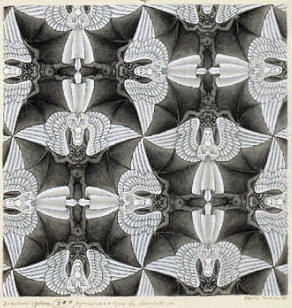
\includegraphics[scale=1]{img/Angel-Devil-1941.eps}
 %\captionsetup{labelformat=empty}
 \caption{Escher, Angles and Devils, 1941}
 \label{fig:Angel-Devil-1941}
\end{figure}
%\end{wrapfigure}

Gödel's first and second incompleteness theorems ended a half-century of attempts, beginning with the work of Frege and culminating in Principia Mathematica and Hilbert's formalism, to find a set of axioms sufficient for all mathematics. Even the elementary arithmetic system is consistent, such consistency cannot be proved within itself. As the great mathematician André Weil said: ``God exists since mathematics is consistent, and the Devil exists since we cannot prove it.''\cite{HanXueTao16}

\section{Proof sketch for the first incompleteness theorem}

按照希尔伯特规划,首先是把整个数学理论组织成一个形式系统。然后在元数学中对这一形式系统进行研究。为此我们需要把古典数学的每一分支表述为这样的形式系统。其中只包含有限条公理,然后通过元数学证明这样的系统是完备的且无矛盾的。其中最基本的一个系统就是自然数算术,因为很多数学系统都同构于它。在上一章,我们看到了如何从自然数出发定义出整数,有理数,甚至实数。从实数对应到点,我们又可以利用解析几何把欧几里得几何算术化。

\subsection{构建形式系统}
\index{TNT系统} \index{印符数论}
这里我们采用侯世达在《哥德尔,埃舍尔,巴赫——集异璧之大成》中的方法和术语来简要介绍这一证明过程。哥德尔不完全性定理的证明也是从构建形式系统开始的。我们称这一系统为“印符数论”简称TNT\footnote{印符数论的英文Typographical Number Theory首字母的缩写。}。恰巧这也是黄色炸药三硝基甲苯的分子式,暗示其威力大到足以——摧毁自己这座大厦。所谓印符数论,就是把用我们熟悉的自然语言表示的数论形式化为一系列印刷字符。这看起来很复杂,但是在我们第一章中介绍的皮亚诺公理的基础上,其实并不难。首先我们要定义数字,按照皮亚诺公理,零是自然数,每个自然数都有其后继,我们很自然地可以这样定义数的印符:

\begin{tabular}{|r|l|}
零 & 0 \\
\hline
一 & S0 \\
\hline
二 & SS0 \\
\hline
三 & SSS0 \\
\hline
…… & …… \\
\end{tabular}

其中符号S代表后继,两个S表示后继的后继。一百个S和一个0表示0的一百次后继,也就是自然数100。尽管很长,但是规则异常的简单。定义了自然数,我们还要定义变量,为了是系统尽量简单,我们可以仅使用5个印符字母$a, b, c, d, e$。当需要更多变量时我们就加撇号,$a', a'', a'''$。接下来我们需要加法符号“$+$”和乘法符号“$\cdot$”以及辅助运算顺序的左右括弧。为了形式化命题我们需要等号“$=$”,表示否定的$\lnot$,表示蕴含的箭头$\to$。这样我们就可以表示命题了,例如(先不论命题的真假):

\begin{itemize}
\item 一加二等于四:$(S0 + SS0) = SSSS0$
\item 二加二不等于五:$\lnot (SS0 + SS0) = SSSSS0$
\item 如果1等于0,那么0等于1:$(S0 = 0) \to (0 = S0)$
\end{itemize}

一个命题中可以含有自由变元,例如:

\[
(a + SS0) = SSS0
\]

表示$a$加上2等于3。显然$a$的取值决定这个命题的真假,为此我们还需要引入存在量词符号$\exists$和全称量词符号$\forall$,以及表示量词约束关系的的冒号“:”。这样命题:

\[
\exists a : (a + SS0) = SSS0
\]

就表示:存在$a$使得$a$加上2等于3。再看另一个例子:

\[
\forall a : \forall b : (a + b) = (b + a)
\]

这恰好就是自然数的加法交换律。如果去掉$a$的量词约束,就变成:

\[
\forall b : (a + b) = (b + a)
\]

这是一个开公式,其中$a$是自由变元。它表示未指定的$a$可以与$b$交换。当然这一命题的真假并没有确定。为了把命题复合起来,我们还需要析取符号$\land$,合取符号$\lor$。尽管TNT中的符号极少,可是它的表达能力却很强,我们举一些例子看:

2不是任何数的平方:$\lnot \exists a : (a \cdot a) = SS0$

费马大定理在$n$为3时成立:$\lnot \exists a : \exists b : \exists c : ((a \cdot a) \cdot a) + ((b \cdot b) \cdot b) = ((c \cdot c) \cdot c)$

现在,我们只是有了可以表示命题的印符,为了构建TNT形式系统,我们还需要公理和推理规则。

\subsubsection{公理和推理规则}

仿照皮亚诺算术的公理,我们为TNT系统定义下述的公理:

\begin{enumerate}
\item $\forall a : \lnot Sa = 0$,这条公理说,没有任何自然数是零的后继;
\item $\forall a: (a + 0) = 0$,这条公理表示任何数加零都等于它本身;
\item $\forall a: \forall b: (a + Sb) = S(a + b)$,这条公理定义出了自然数的加法;
\item $\forall a: (a \cdot 0) = 0$,这条公理表示任何自然数乘以零都为零;
\item $\forall a: \forall b: (a \cdot Sb) = ((a \cdot b) + a)$,这条公理定义出自然数的乘法。
\end{enumerate}

接下来我们构建推理规则。比如我们希望从公理1,零不是任何自然数的后继这一普通情况,导出1不是零的后继这一特殊情况,为此我们需要引入特称规则:

\textbf{特称规则}:如果$u$是出现在印符串$x$中的变元。如果$\forall u: x$是一个定理,则$x$也是定理,并且对$x$中的$u$做任何替换得到的新印符串也是定理。

这里有一个限制,在替换$u$时,不能包含任何$x$中被量化的变元,并且替换要一致。与特称规则相反的是概括规则。这个规则允许我们把全称量词加到定理的前面。

\textbf{概括规则}:如果$x$是一个定理,其中的变元$u$是自由出现的。则$\forall u: x$也是一个定理。

例如,$\lnot S(c + S0) = 0$,表示不存在一个数加一的后继等于零,我们可以概括为:$\forall c: \lnot S(c + S0) = 0$。

接下来的规则可以让我们把全称量词和存在量词互换。

\textbf{互换规则}:如果$u$是一个变元,那么印符串$\forall u: \lnot $与$\lnot \exists u:$可互换。

例如公理1可以按照互换规则变成:$\lnot \exists a: Sa = 0$。接下来的一个规则允许我们在一个印符串的前面加上存在量词。

\textbf{存在规则}:假设一个项在定理中出现一次或多次,可以用一个变元来代替这个项,并且在前面加上存在量词。

我们还用公理1来举例:$\forall a: \lnot Sa = 0$中,我们可以把0,用变元$b$来代替,并且在前面加上存在量词。这样就得到:$\exists b: \forall a: \lnot Sa = b$。意思是说,存在一个数,使得任何自然数都不是它的后继。

接下来考虑相等的对称性和传递性,我们定义等号规则。令$r, s, t$都代表任意的项。

\textbf{等号规则}:
\begin{itemize}
\item 对称:如果$r = s$是定理,则$s = r$也是定理;
\item 传递:如果$r = s$和$s = t$都是定理,则$r = t$也是定理。
\end{itemize}

对于增、减后继符号$S$,我们也定义一个规则。

\textbf{后继规则}:
\begin{itemize}
\item 增加:如果$r = t$是定理,则$Sr = St$也是定理;
\item 去除:如果$Sr = St$是定理,则$r = t$也是定理。
\end{itemize}

现在的印符数论TNT已经很强大了,我们可以用它构造出各种比较复杂的定理。

\begin{Exercise}
\Question{尝试给出费马大定理的印符串。}
\Question{尝试用印符推理规则证明加法结合律。}
\end{Exercise}

\subsubsection{印符系统的不完全性}

使用TNT系统中的公理和推理规则不难证明下面的一系列定理:

\[
\begin{array}{rcl}
(0 + 0) & = & 0 \\
(0 + S0) & = & S0 \\
(0 + SS0) & = & SS0 \\
(0 + SSS0) & = & SSS0 \\
... & & ...
\end{array}
\]

第一条可以从公理2中,把$a$代换成0导出;第二条可以用公理3和上一条定理导出,每条定理都可以从上一条定理轻松导出。作为旁观者的我们,立刻想到这能不能概括成一条定理:

\[
\forall a: (0 + a) = a
\]

请注意它和公理2的区别。遗憾的是,利用迄今为止所给出的TNT规则,我们无法导出这一定理。我们也许希望添加一条规则,如果一系列这样的串都是定理,那么概括它们的全称量词串也是定理。但是这条规则只有在系统外部的人才能洞见。它不是一条可以放入形式系统的规则。

\index{omega不完全}
缺少这样的概括能力说明印符数论系统TNT是不完全的,确切地说,叫作$\omega$不完全的。这里的$\omega$恰恰就是上一章介绍的可数无穷基数。我们说一个系统是$\omega$不完全的,如果一系列无穷的串都是定理,而其全称概述却不是定理。并且更奇特地,这一印符串的否定形式:

\[
\lnot \forall a: (0 + a) = a
\]

也不是TNT中的定理。这意味着这个串在TNT中是不可判定的。这只是说TNT的能力不足以判定这个串是否是定理。就如同利用欧几里得几何的前四条公设无法判定第五公设一样。我们或者加入第五公设构成欧几里得几何;或者加入第五公设的否定构成非欧几何。我们可以将这一印符串或者其否定加入到TNT中,构造出不同的形式系统。

如果我们选择了这一印符串的否定,这里看似奇怪的一点是,零加上任何数都不再等于这个数了。这和我们通常熟悉的自然数加法大相径庭。但这恰恰提醒我们,所谓形式系统是带有未定义项的。我们只是方便理解选择了加号和自然数的含义。

印符系统TNT的$\omega$不完全性提示我们,我们的系统还缺少一条重要的规则——读者也许想到了——代表数学归纳法的皮亚诺第五公设。为此我们添上最后一块拼图。

\textbf{归纳规则}:如果$u$是印符串$X$中的一个变元,记为$X{u}$。如果把$u$替换为0时成立,且有$\forall u: X{u} \to X{Su}$。也就是若$u$时$X$成立,则将$u$替换为$Su$时$X$也成立。那么$\forall u: X{u}$是一个定理。

加上数学归纳法后,印符数论系统TNT终于和皮亚诺算术具有同样的能力了。

\begin{Exercise}
\Question{利用新加入的归纳规则证明$\forall a: (0 + a) = a$}
\end{Exercise}

\subsection{哥德尔配数}
\index{哥德尔配数}
哥德尔证明的最关键一步是引入了哥德尔配数。TNT系统已经强大到可以反映其它形式化系统,有没有可能利用TNT系统谈论它自身呢?哥德尔想到的办法就是把推理规则进行“算术化”。为此他把所有符号分配了一个数。

\begin{table}[htbp]
\centering
\begin{tabular}{|l|r||l|r|}
\hline
\textbf{符号} & \textbf{数} & \textbf{符号} & \textbf{数} \\
\hline
0 & 666 & S & 123 \\
\hline
= & 111 & + & 112 \\
\hline
$\cdot$ & 236 & ( & 362 \\
\hline
) & 323 & $a$ & 262 \\
\hline
$'$ & 163 & $\land$ & 161 \\
\hline
$\lor$ & 616 & $\to$ & 633 \\
\hline
$\lnot$ & 223 & $\exists$ & 333 \\
\hline
$\forall$ & 626 & : & 636 \\
\hline
\end{tabular}
\caption{对TNT系统进行哥德尔配数的一种方法}
\end{table}

这样公理1就可以做如下的翻译:

\begin{tabular}{cccccccc}
$\forall$ & $a$ & : & $\lnot$ & $S$ & $a$ & = & 0 \\
626 & 262 & 636 & 223 & 123 & 262 & 111 & 666 \\
\end{tabular}

配数的方法并不唯一。经过这样的配数,TNT中的任何串都可以表示为一个数了(尽管非常大)。现在问题来了,任给一个数,我们有没有办法判断它是一个TNT定理所代表的数呢?我们知道最开始有5个数一定是TNT数。它们就是五条公理所代表的数。根据TNT的推理规则,从这5个数开始,可以构造出无穷无尽的TNT数。在此之上我们引入一个数论谓词:

\begin{center}
$a$是个TNT数。
\end{center}

例如626,262,636,223,123,262,111,666是个TNT数(这里的逗号只是为了方便读写,和英文中每三位一分隔是同样的)它表示公理1。其否定形式是:

\begin{center}
$\lnot a$是个TNT数。
\end{center}

例如我们说123,666,111,666不是个TNT数。这意味着我们可以把$a$替换成0后面跟着123666111666个S。而这个巨大的串的含义实际是:$S0 = 0$不是TNT的定理。这意味着,TNT的确可以谈论它自己。这不是一种巧合,而是源于任何形式系统都可以在数论$N$中得到反映。于是我们形成了一个圈:形式系统TNT中的一个串有一个数论$N$中的解释,而$N$中的一个陈述可以有第二层含义,就是作为元语言对TNT的陈述。

\begin{figure}[htbp]
\centering
\begin{tikzpicture}[scale=0.8]
\draw (-5, 0) circle[x radius=1.5cm, y radius=1cm] node (TNT) {TNT}
      (0, 0) circle[x radius=1.5cm, y radius=1cm] node (N) {数论$N$}
      (5, 0) circle[x radius=1.5cm, y radius=1cm] node (Meta-TNT) {元TNT};
\draw[->] (TNT) to node [above] {数论解释} (N);
\draw[->] (N) to node [above] {元语言陈述} (Meta-TNT);
\end{tikzpicture}
\caption{TNT $\to$ 数论$N$ $\to$ 元TNT}
\label{fig:TNT-N-TNT}
\end{figure}

\subsection{构造自我指涉}

哥德尔做的最后一步是构造一个自我指涉。找到一个TNT串,称之为$G$,它是关于它自己的。其意义为:

\begin{center}
$G$不是TNT的定理
\end{center}

接下来我们可以引爆TNT了。那么究竟$G$是否是TNT中的定理呢?如果$G$是一个定理,那么它表示的就是真理,即:“G不是定理”。我们看到自指命题的威力了。由于充当了定理,$G$就不得不是个假理。根据我们的假定,TNT不会把假理当作定理,于是我们被迫得出结论说$G$不是个定理。但是知道了$G$不是个定理后,我们就得承认$G$表示了一个真理。这揭示出TNT没有达到我们的期望——我们发现了一个符号串,它表示了真理,然而却不是一个定理。但考虑$G$还有一个算术解释这一事实。它表示了关于自然数的某个算术性质的一个陈述。通过在TNT系统外面进行的推理,我们确定了这个陈述为真,还确定了这个串不是TNT的定理。我们问TNT这个串是否为真,TNT将既不能说“是”,也不能说“不”。

$G$就是那个不可判定命题。这就是哥德尔不完全定理的证明思路。

\section{万能的程序与对角线证明}
\index{原始递归函数}
哥德尔不完全性定理对于编程意味着什么呢?我们有一个在编程上完全同构的问题。为此,我们从设计一个形式化的计算机语言开始。这个语言支持原始递归函数。所谓原始递归函数是一类数论函数,它们可以从自然数映射到自然数,并遵循下面5条公理:

\begin{enumerate}
\item 常函数:0元常函数0是原始递归的;
\item 后继函数:一元后继函数$S(k) = k + 1$是原始递归的;
\item 投影函数:传入$n$个数,返回其中第$i$个数的函数$P_i^n$是原始递归的;
\item 组合:原始递归函数的有限次组合是原始递归的;
\item 原始递归:
\[
\begin{cases}
h(0) = k \\
h(n + 1) = g(n, h(n)) \\
\end{cases}
\]
称$h$是由$g$经原始递归运算得到的,可以扩展到多元的情况。
\end{enumerate}

包含加、减基本运算符号、条件分支(if-then)、等于、小于判断和有界循环的编程语言被称为原始递归的编程语言。所谓有界循环指循环的次数在进入循环体前是确定的。它可以是不带跳转语句(goto)的loop,或者是在循环体中不能改变循环变量的for循环。但不能是while循环或repeat-until循环。由于这些限制,所有原始递归的程序必然是确定停机的。

原始递归函数的一个重要性质是全部原始递归程序是递归可枚举的。假设我们可以从全部原始递归程序中筛选出那些只有一个输入一个输出程序,把它们列出,放入到一个无穷大的程序库里。我们给每个程序一个编号\footnote{其中一种编号方案是把程序文字的ASCII码连接起来形成一个数,然后把这些数从小到大排列。由于没有两个程序是相同的,所以其ASICII码形成的数也不同。},从自然数0开始,1,2,3……一直枚举下去。我们可以把这些程序记为$B[0], B[1], B[2], ...$。对于第$i$个程序,输入参数数$n$时得到结果是$B[i](n)$。

现在,我们构造这样一个特殊的函数$f(n)$,当输入$n$时,它的输出恰好是编号为$n$的那个程序,当输入等于$n$时的值加上1,即:

\[
f(n) = B[n](n) + 1
\]

这样的$f$显然是可计算的。我们现在问,$f$是一个存储在函数库中的原始递归程序么?如果是,假设它在程序库中的编号是$m$,根据我们之前的定义,第$m$个程序输入$m$时的结果应该是$B[m](m)$。可是根据$f$的定义,它的输出结果又应该是$f(m) = B[m](m) + 1$。这两个结果显然不相等。这就证明了存在不是原始递归的可计算函数。

这个证明方法和上一章介绍的康托尔对角线证明法如出一辙。因此我们被迫放弃有界循环的限制来扩展编程语言的能力。我们可以引入带有跳转的loop循环,可以在循环体中改变循环变量的for循环,while循环,repeat-until循环,以及可递归的函数。这样就从原始递归函数扩展到了全递归函数。这样的语言称为图灵完备的语言。人们创造的大多数计算机语言都是图灵完备的,可以同构到自然数算术这样的形式系统中。但图灵完备的语言仍然存在漏洞,因为我们可以构造出判断停机的原始递归程序,从而证明存着这不可计算问题。有没有可能进一步放宽限制,增强图灵完备语言,从而设计出万能的程序么?答案是否定的,图灵完备语言已经达到了最高级别,也就是形式系统的极限,没有其他限制可以去掉了。哥德尔不完全性定理告诉我们,形式系统一旦强大到足够的程度,可以包含自然数算术,那么它就必然存在不可判定命题。

\section{尾声}

\begin{wrapfigure}{R}{0.6\textwidth}
%\begin{figure}[htbp]
 \centering
 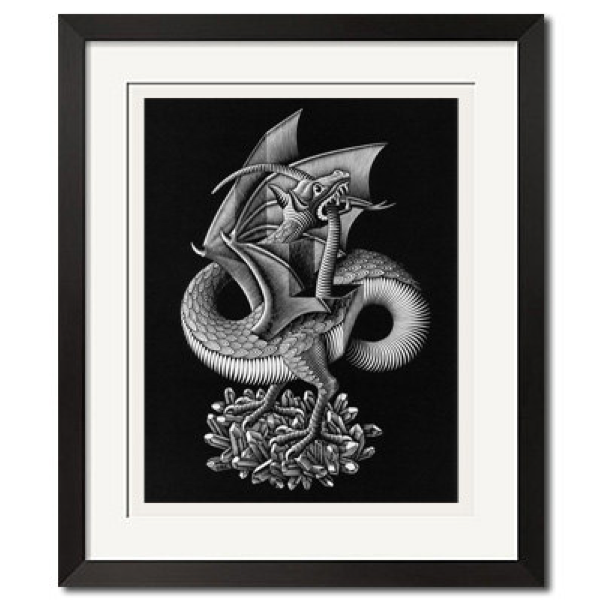
\includegraphics[scale=0.8]{img/Escher-Dragon.eps}
 %\captionsetup{labelformat=empty}
 \caption{埃舍尔《龙》}
 \label{fig:Escher-Dragon}
%\end{figure}
\end{wrapfigure}

我们的理性思维是伟大的。它可以跨越千年,与古代的先哲对话;它可以跨越宇宙,思考我们足迹无法踏上的天体;它可以预见出肉眼看不见的基本粒子;它可以突破直觉,到达高维度的神奇世界。仰望天空,无论是天高云淡,还是月朗星稀,我们也会感叹自身的渺小,在浩瀚的时间长河中,我们不过是匆匆的过客,犹如沧海一粟。

本章我们探讨的问题,究其实质是人类自身的问题。我们的理性思维是否存在边界?我们是否在沿着一个怪圈吞噬着自己?在人工智能突飞猛进发展时,这是每个人都会思考的问题。人类在试图用机器同构自己,用巨大的计算资源同构我们的大脑和理性思维。这就如同埃舍尔作品中的龙,它奋力想从二维世界中挣脱出来,它自己觉得已经把画纸的中部剪开一个缺口,并把尾巴伸了出来。这条龙一口咬住自己的尾巴,拼命想把自己拉到三维的世界中去。作为旁观者的我们,却明明白白知道所有的这一切,仍然在二维的纸张上。这条龙的努力是徒劳的。所有这一切,皆是虚妄、如雾亦如电、当作如是观。

一百年前的激烈讨论和哥德尔的天才证明,在今天依然有着现实意义。作为人类,我们心怀敬畏,敬畏自然,敬畏宇宙,敬畏我们祖先,也敬畏我们自身。

\ifx\wholebook\relax \else
\begin{thebibliography}{99}

\bibitem{Gatys-2015}
Leon A. Gatys, Alexander S. Ecker, Matthias Bethge. ``A Neural Algorithm of Artistic Style.'' 2015. arXiv:1508.06576 [cs.CV] IEEE Conference on Computer Vision and Pattern Recognition (CVPR) 2017.

\bibitem{GuSen-2012}
顾森 《思考的乐趣——Matrix67数学笔记》 人民邮电出版社,2012年,ISBN: 9787115275868

\bibitem{SICP}
Harold Abelson, Gerald Jay Sussman, Julie Sussman 著 裘宗燕 译 ``计算机程序的构造和解释(原书第二版)''. 北京 机械工业出版社 2004年 ISBN: 7-111-13510-5

\bibitem{HanXueTao16}
韩雪涛 ``数学悖论与三次数学危机''. 人民邮电出版社. 2016, ISBN: 9787115430434

\bibitem{M-Kline-2007}
[美] M$\cdot$克莱因 著 李宏魁 译 ``数学:确定性的丧失'' 湖南科学技术出版社,2007年4月 ISBN: 978-7-5357-1857-0
% Morris Kline ``Mathematics: The Loss of Certainty''. Oxford University Press, 1980.

\bibitem{Poincare2}
[法]彭加勒 著,李醒民 译 ``科学的价值'' 商务印书馆. 2010 ISBN: 978-7-100-07045-4

\bibitem{Ried-1996}
Constance Ried. ``Hilbert''. Springer, 1st Printing edition, 1996, ISBN: 978-0387946740

\end{thebibliography}

\expandafter\enddocument
%\end{document}

\fi
